\chapter{Design of a Mitosis Detection algorithm}
\label{chapter4}
\thispagestyle{empty}

\begin{quotation}
{\footnotesize
\noindent \emph{\textquotedblleft Ab uno\\ disces omnis\textquotedblright}\\
\noindent (Learn everything from one)
\begin{flushright}
Publius Vergilius Maro (Aeneis II, 65-66)
\end{flushright}
}
\end{quotation}

\vspace{0.5cm}

%\noindent In questa sezione si spiega come \`e stato affrontato il problema concettualmente, la soluzione logica che ne \`e seguita senza la documentazione.

We developed an algorithm to perform mitosis-detection as a part of our work, with the aim to compare its results with humans facing the same task.

\section{Dataset}
\label{ch4:ds}

We used the public MITOS dataset \cite{icpr}. The dataset is composed by a total of 50 2084$\times$2084 pixel images
covering an area of 512$\times$512 $\mu$m each, acquired with an APERIO XT scanner (see Figure \ref{ch2:fig1}). 
A unique split is defined by the dataset authors, with 35 images used for training and 15 for evaluation.
The dataset contains a total of about 300 mitosis, which were annotated by an expert pathologist.
The performance of the algorithms participating to the \textit{2012 ICPR mitosis detection contest} are shown in Section \ref{ch3:icpr_perf}.\\
With reference to Figure \ref{ch3:fig1}, we focused on on the classification subproblem, with the \Glspl{ROI} given as an input.
The input is given in form of an image patch with size 100$\times$100 pixel: such size completely contains the image of the cell.
The task is to map each patch to one of two classes:
\begin{itemize}
 \item [] \textit{\textbf{C1}}: the image contains a mitosis at its center,
 \item [] \textit{\textbf{C0}}: the image does not contain a mitosis anywhere. 
\end{itemize}

There are no samples in which a mitosis is visible off-center.

\vspace{0.5cm}

\subsection{Image Candidates}
\label{ch4:ic}

For the \textit{\textbf{C1}} class, all the 216 mitosis available in the 35 training images are chosen
as training samples, and all 87 mitosis in the evaluation images are chosen as
evaluation samples.\\
We enforced an even distribution of the two classes classes both in training and in evaluation sets, and therefore
selected 216 \textit{\textbf{C0}} samples for training, and 87 \textit{\textbf{C0}} samples for evaluation; the resulting
training set contained 432 samples.\\
Millions of different \textit{\textbf{C0}} samples may be randomly chosen from the original training and evaluation images:
an overwhelming majority of such samples would not contain any nucleus and be non-informative for training and trivial for
evaluation. Limiting the choice to non-mitotic nuclei \texttwelveudash{} which greatly outnumber
mitotic ones \texttwelveudash{} would not solve the problem, since most of such nuclei look very
similar to each other and are trivially identified as non-mitotic. Only a small
subset of non-mitotic nuclei \texttwelveudash{} as well as other structures and artifacts \texttwelveudash{} pose an
actual challenge, both for humans and for algorithms.\\
In order to select such objects as \textit{\textbf{C0}} samples, we used the output produced by a simple \Gls{CNN}-based mitosis detector,
similar to the one outlined in \cite{agNN} for selecting useful training samples.
The detector, built at IDSIA, was trained on few images in the training set, then applied on the whole dataset.
Because the detector was simple and trained on a small amount of data, it performed poorly and detected a lot of false positives.
\textit{\textbf{C0}} samples have been randomly chosen among the outputs of such detector which are
farther than 50 pixels from the centroid of any mitosis; this ensures that no actual
mitosis is visible in the corresponding image patch. The resulting samples do in
fact resemble mitosis, are informative in the training set, and appear non-trivial
in the evaluation set. Finally, 10 \textit{\textbf{C0}} samples in the evaluation set are substituted
with 5 random false positives obtained from each of the two best performing
algorithms (IDSIA and IPAL). These last 10 samples are particularly useful to compare humans to algorithms, in fact allowed us to better observe how test subjects
behave on the algorithms’ false positives, which are rare in the evaluation set because
algorithms were tuned to solve a problem with very low prevalence of mitotic samples.


\vspace{0.5cm}

\subsection{Extended Dataset}
\label{ch4:ed}

We extended our dataset by rotating and mirroring each image patch (see Figure \ref{ch4:fig1}). We used the extended dataset only for the detection algorithm, so that we could analyze
the effect of different features, which can be explicitly dependent on orientation or not, on the global performance of the classifier.\\
In case of extended dataset, the classification of a single image patch becomes the average of the classifications obtained on the 8 samples.

\begin{equation}
 c_{i} = \frac{\sum_{j=1}^{8} c_{ij}}{8}
\end{equation}

Where $c_{i}$ represents the classification of image patch \textit{i}, and $c_{ij}$ represents the classification of variation \textit{j} of image patch \textit{i} .



\begin{figure}[!hbt]
  \centering
    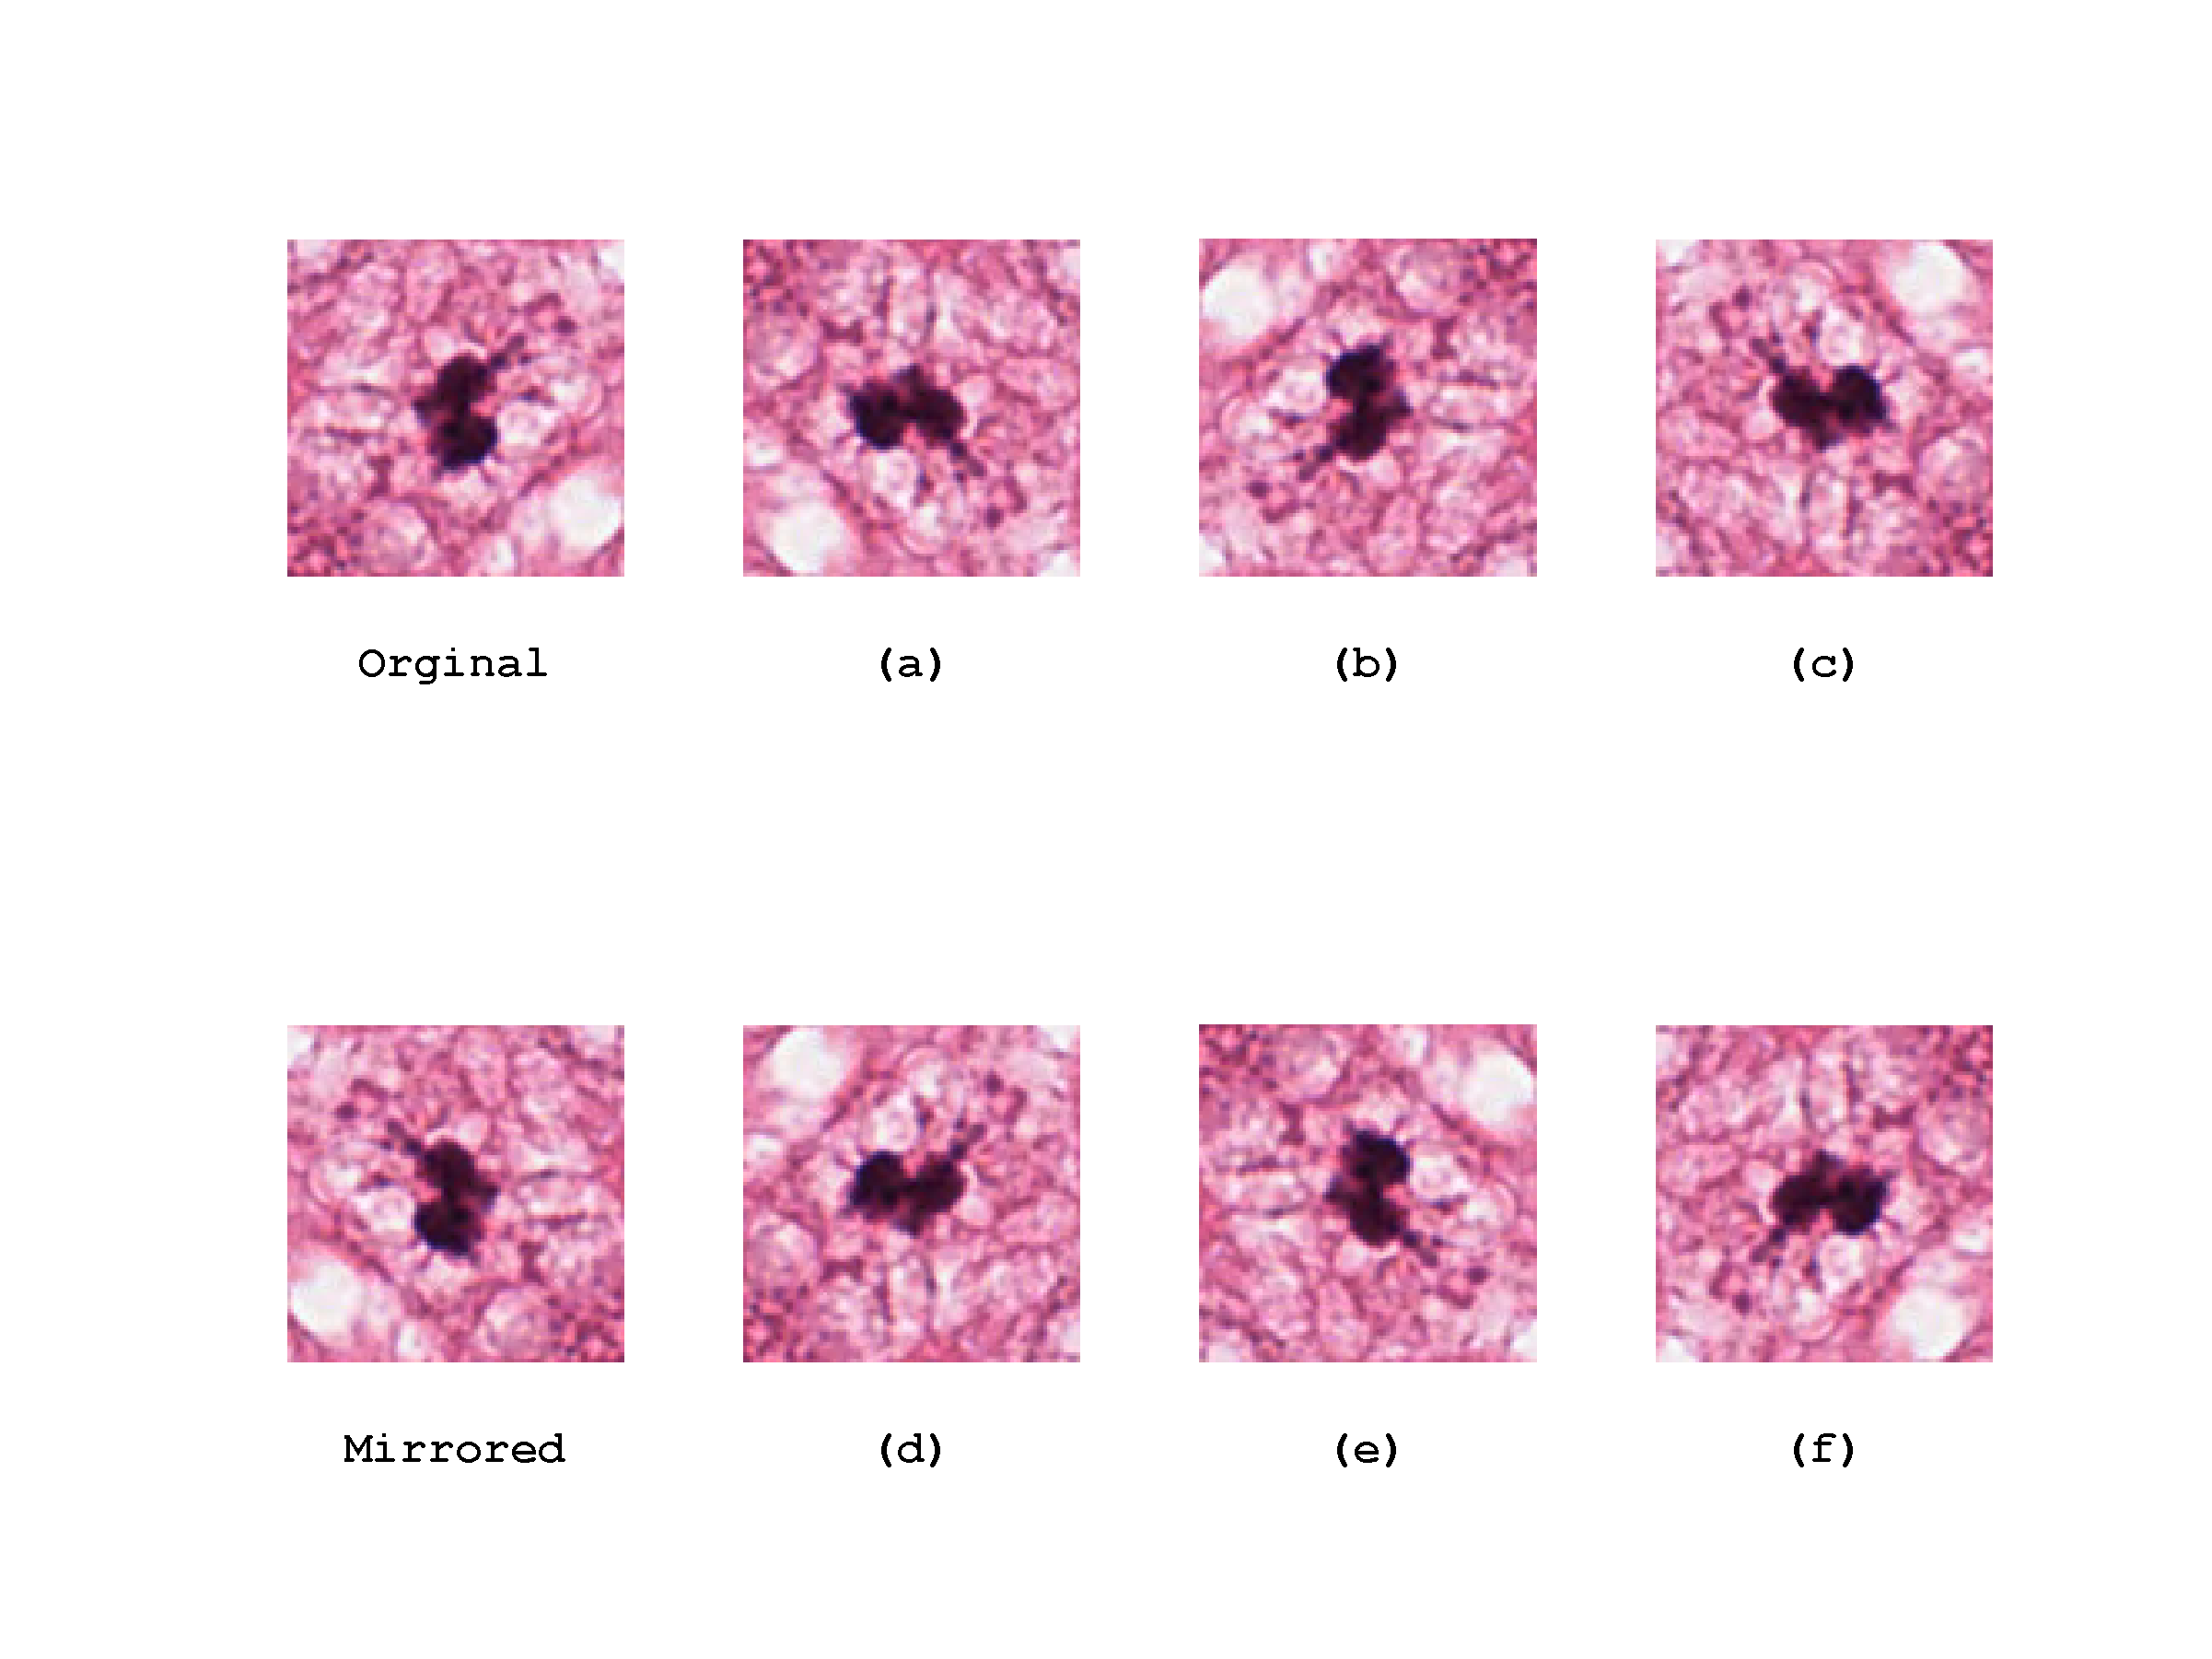
\includegraphics[width=0.94\textwidth]{./images/rotDataset.png}
  \caption[Extended Dataset]{Extended dataset\\(a),(b),(c): $\pi/2$ clockwise rotations, (d),(e),(f): mirror and $\pi/2$ clockwise rotations.}
  \label{ch4:fig1}
\end{figure}  

\vspace{0.5cm}




\section{Features Extraction}
\label{ch4:FE}

Each image patch can be represented as a 100$\times$100$\times$3 matrix, where the $(i,j,:)$ triplet represents the RGB value of point with coordinates $(i,j)$ in the image.
Each value is in the range 0 to 255. Starting from these (raw) data we extracted some features by which we trained and tested our classifiers.

\vspace{0.5cm}

\subsection{Simple Features}
\label{ch4:sf}

The simplest features that can be computed involve the average and the standard deviation of the \Gls{RGB} values of the image patch. They can be computed on all the data or can be maintained separated
for each \Gls{RGB} component. In the first case, average and standard deviation each give one value every instance:

\begin{eqnarray}
 m & = & \frac{1}{100\cdot100\cdot3} \left( \sum_{i=1}^{100} \sum_{j=1}^{100} \sum_{k=1}^{3} i_{ijk} \right) \\
 \sigma & = & \sqrt{\frac{1}{100\cdot100\cdot3} \left( \sum_{i=1}^{100} \sum_{j=1}^{100} \sum_{k=1}^{3} (i_{ijk} - m )^2 \right)}
\end{eqnarray}

Otherwise, average and standard deviation produce a vector of three components:

\begin{eqnarray}
 \overline{M} & = & \left[ \begin{array}{c}
                            \frac{1}{100\cdot100} \left( \sum_{i=1}^{100} \sum_{j=1}^{100} i_{ij1} \right) \\
                            \frac{1}{100\cdot100} \left( \sum_{i=1}^{100} \sum_{j=1}^{100} i_{ij2} \right) \\
                            \frac{1}{100\cdot100} \left( \sum_{i=1}^{100} \sum_{j=1}^{100} i_{ij3} \right)
                           \end{array} \right] \\
 \overline{S} & = & \left[ \begin{array}{c}
                                 \sqrt{\frac{1}{100\cdot100} \left( \sum_{i=1}^{100} \sum_{j=1}^{100} (i_{ij1} - M(1) )^2 \right)} \\
                                 \sqrt{\frac{1}{100\cdot100} \left( \sum_{i=1}^{100} \sum_{j=1}^{100} (i_{ij2} - M(2) )^2 \right)} \\
                                 \sqrt{\frac{1}{100\cdot100} \left( \sum_{i=1}^{100} \sum_{j=1}^{100} (i_{ij3} - M(3) )^2 \right)}
                                \end{array}  \right]
\end{eqnarray}

Another simple set of features is represented by the \textit{median} of each \Gls{RGB} value. The median is defined as the numerical value separating the higher half of the data sample, from the lower half
and can be found by arranging all the data from lowest value to highest value and picking the middle one, or the mean of the two middle values, in case of even data.
Each of the features above are independent of the orientation of the image.
%	-	m: mean
%	-	s: standard deviation
%	-	M: mean per color
%	-	S: std per color
%	-	d: median per color



\vspace{0.5cm}

\subsection{Color Histograms and Intensities}
\label{ch4:chi}

A color histogram is a representation of the distribution of colors in an image, i.e. the number of pixels that have colors in each of a fixed list of color ranges \cite{colorHistogram01},
that span the image's color space. The color histogram can be built for any kind of color space, although the term is more often used for three-dimensional spaces like \Gls{RGB} or \Gls{HSV}.
A histogram of an image is produced first by discretization of the colors in the image into a number of bins, and counting the number of image pixels in each bin.
We built the \Gls{RGB} color histogram for each image patch, using 16 bins for each channel. The feature vector is so composed of 48 elements.\\
Also this feature is orientation independent.


\begin{figure}[!hbt]
  \centering
    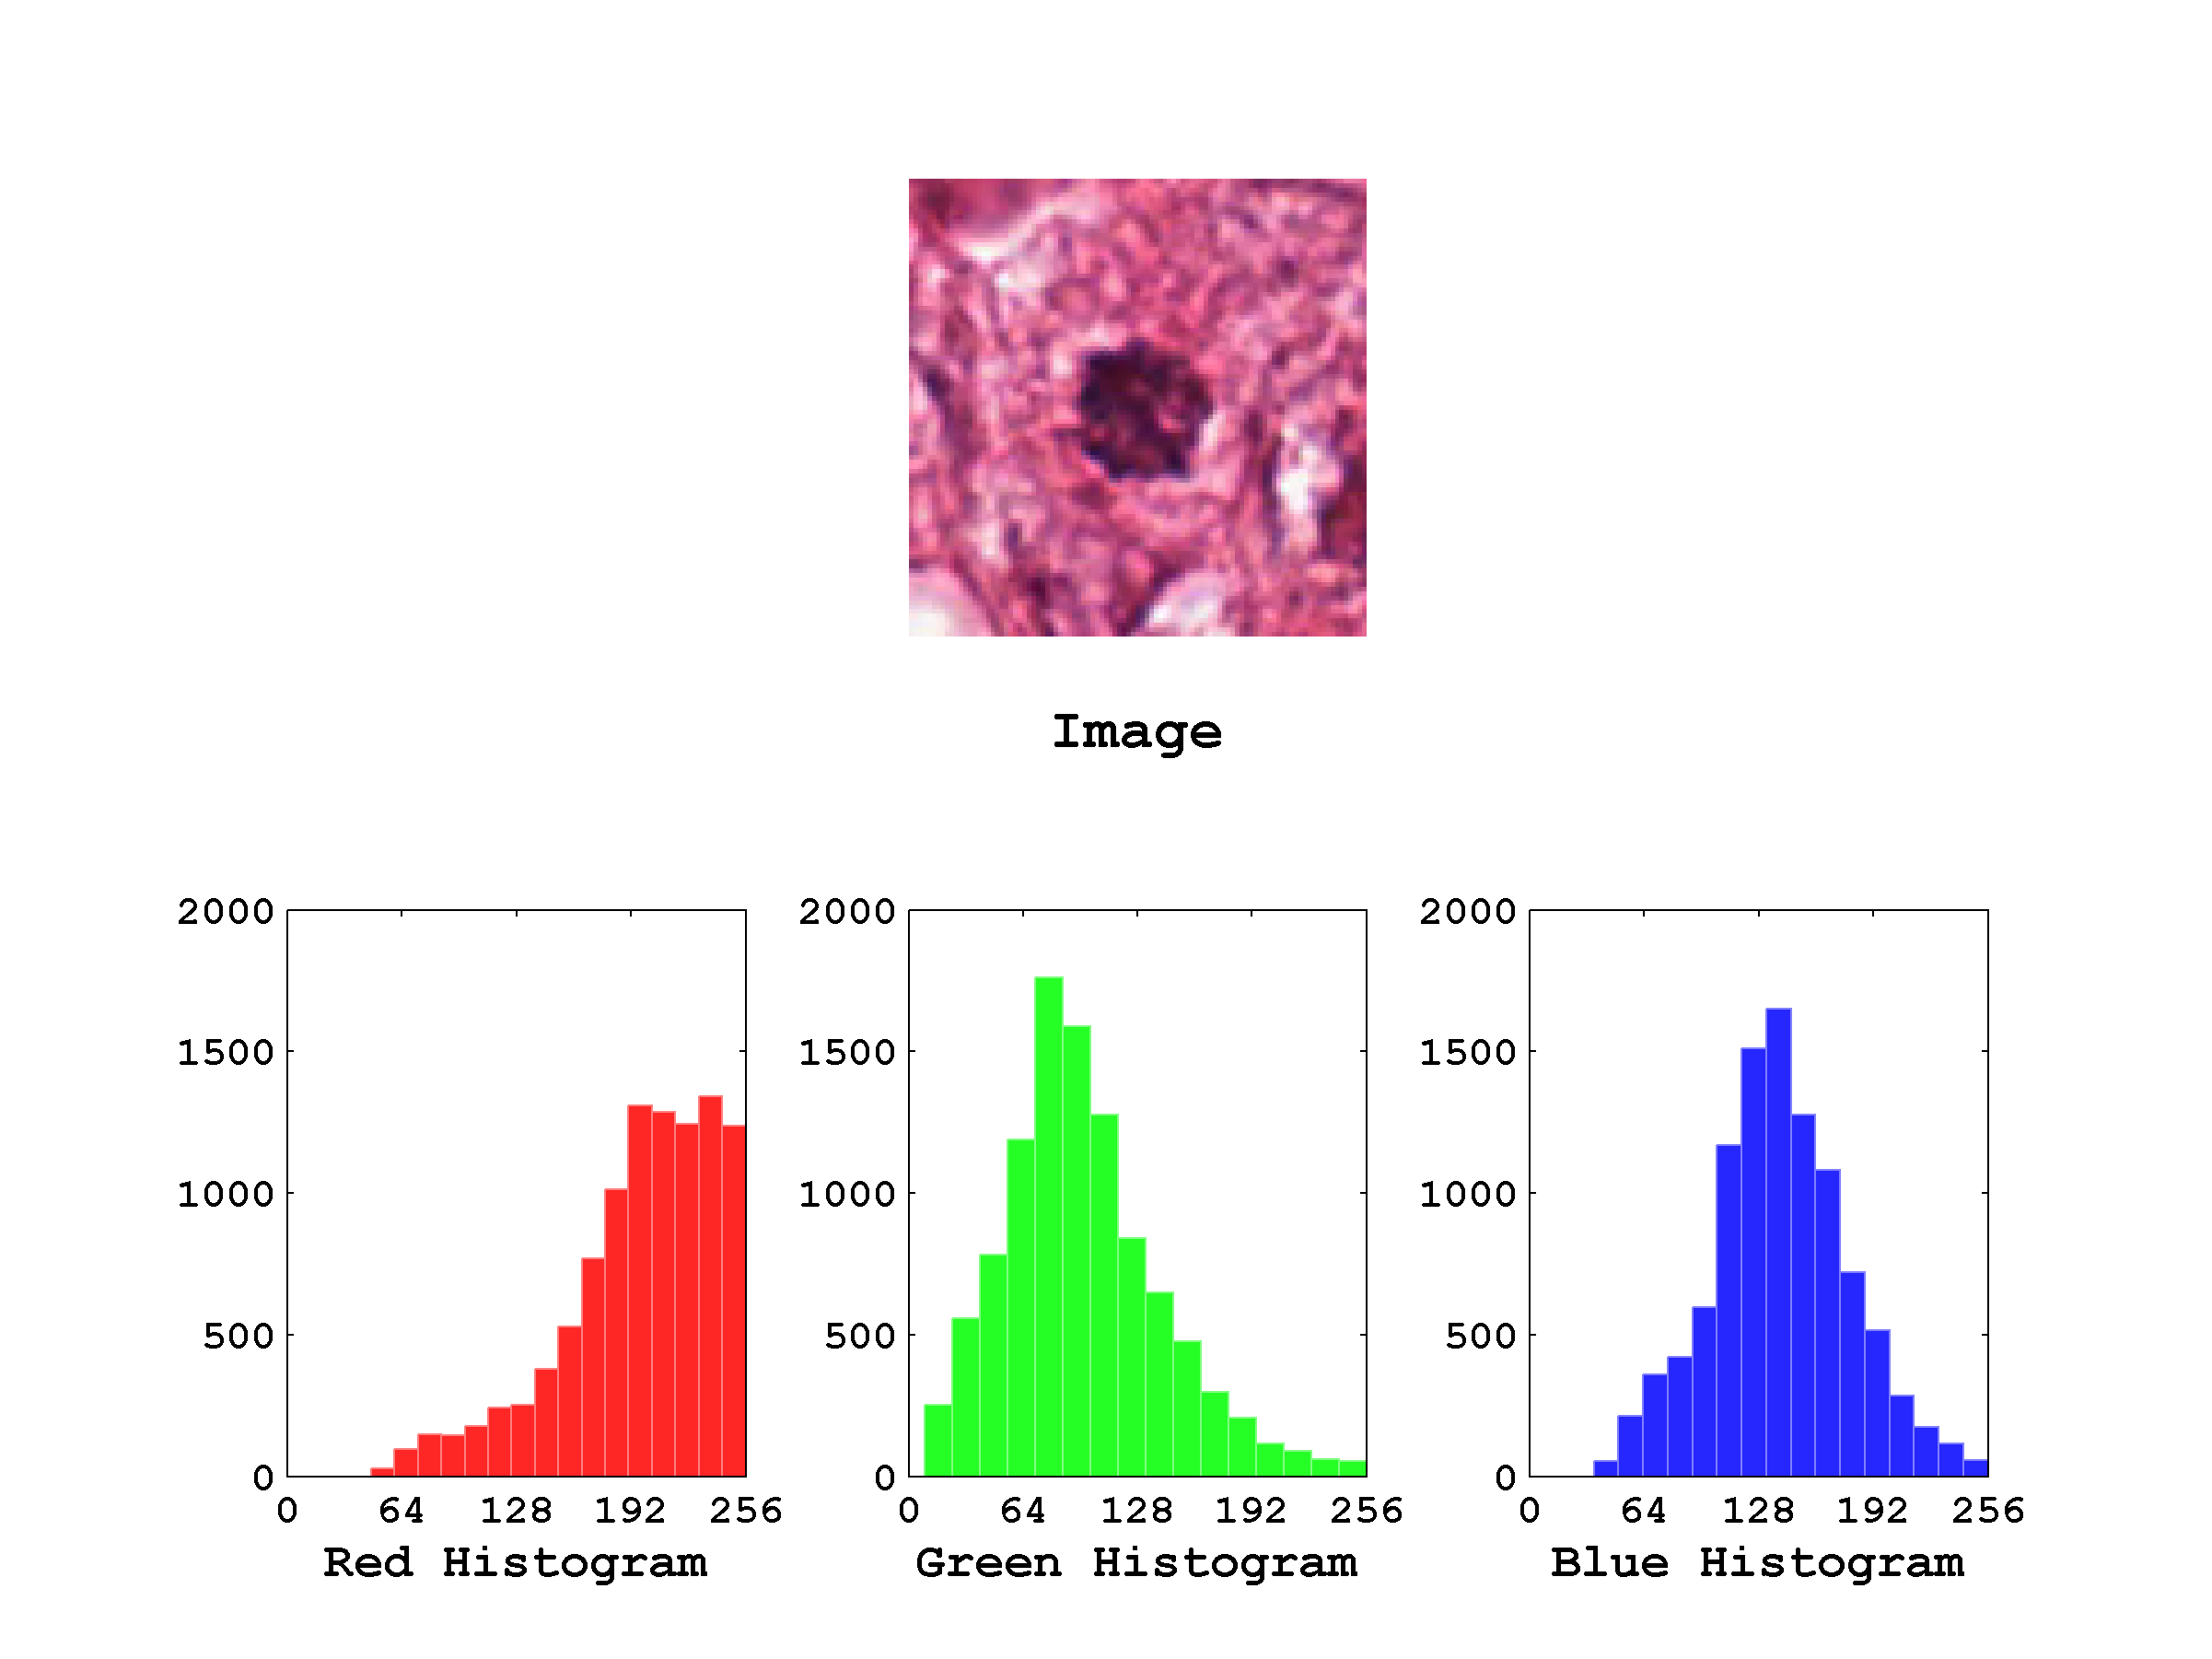
\includegraphics[width=0.94\textwidth]{./images/histIM.png}
  \caption[Color Histograms]{Color Histograms of sample image}
  \label{ch4:fig2}
\end{figure}  

It is generally possible to transform a color image into a gray-scale one. One typical transformation algorithm, applied pixel by pixel, is the following:

\begin{equation}
 \label{ch4:eqGS}
 pix_{gray} = 0.2989 \cdot pix_{red} + 0.5870 \cdot pix_{green} + 0.1140 \cdot pix_{blue}
\end{equation}

On the resulting monochromatic image, it is possible to compute an \textit{intensity histogram}.\\
We preferred to compute a slightly different feature: the average intensity in the 25 central regions of the image.
We first computed the gray-scale image according to Equation \ref{ch4:eqGS}, then we selected the central part of the image and divided it in a grid of $5\times5$ elements.
We finally computed the mean intensity for each element. Figure \ref{ch4:fig3} illustrates the procedure.

\begin{figure}[!hbt]
  \centering
    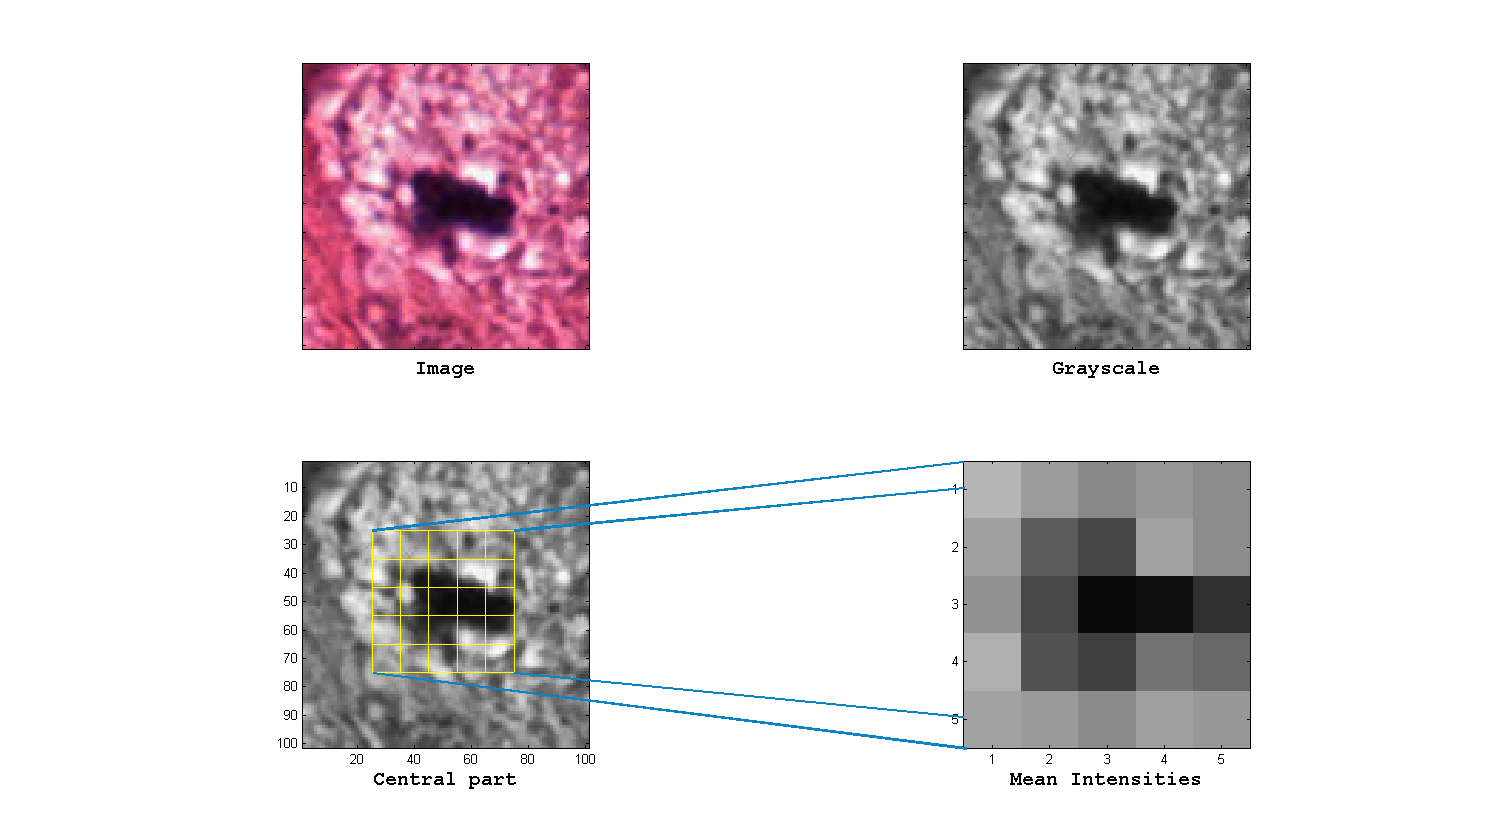
\includegraphics[width=0.94\textwidth]{./images/GSintens1.png}
  \caption[Example of mean gray-scale intensities feature]{Mean gray-scale intensity of central part of image patch}
  \label{ch4:fig3}
\end{figure}

The resulting feature vector is composed of 25 values, corresponding to the intensities, ordered columnwise. This type of feature is orientation dependent.

%	-	H: color histograms (16 bins)
%	-	i: mean intensity in 25 central regions of the image


\vspace{0.5cm}

\subsection{Texture Features}
\label{ch4:tf}

Texture features are widely used in different \Gls{CV} tasks, as pointed out in Section \ref{ch2:texture}. We focused on the features described in \cite{LBP01} and \cite{LBP02},
based on Local Binary Patterns (\Gls{LBP}). The general idea of \Gls{LBP} is described on page \pageref{ch2:lbp}.
The \Gls{LBP} features considered here are labeled LBP$_{P,R}$, where \textit{P} is the number of neighbors considered and \textit{R} is the distance from the pixel.
The two main characteristics of the \Glspl{LBP} considered are:

\begin{itemize}
 \item \textit{uniformity}: which is a fundamental property of local image texture. It refers to the uniform appearance of the local
binary pattern, that is, there is a limited number of transitions or discontinuities in the circular presentation of the pattern.
The most frequent uniform binary patterns correspond to primitive \textquotedblleft microfeatures\textquotedblright, such
as edges, corners, and spots; hence, they can be regarded as feature detectors that are triggered by the best matching
pattern.
\item \textit{rotation invariance}: which takes into account if a spatial pattern is affected by rotation or not.
\end{itemize}

Three different types of features can be built, on the basis of Equation \ref{ch2:eq_lbp1}:

\begin{enumerate}
 \item $\text{LBP}_{P,R}^{u2}$: uniform feature,
 \item $\text{LBP}_{P,R}^{ri}$: rotation invariant feature,
 \item $\text{LBP}_{P,R}^{riu2}$: uniform and rotation invariant feature,
\end{enumerate}

In particular we used:

\begin{equation}
 \text{LBP}_{8,R}^{\text{type}} \quad \textrm{where} \begin{cases}
    \text{type}  & \in \{ri, u2, riu2\}\\
    R  & \in \{1,2,3\}
  \end{cases}
\end{equation}

while building the feature vector, we used the \textit{type} parameter in a mutually exclusive way, i.e. we did not concatenate \Glspl{LBP} of different types. On the other hand, we
built feature vectors with various combitations of radii.\\
The following equations show the three different mutually exclusive texture feature sets that we considered.

\begin{eqnarray}
\label{ch4:tftypes}
 \overline{L} & = & \left[ \text{LBP}_{8,1}^{riu2}, \text{LBP}_{8,2}^{riu2}, \text{LBP}_{8,3}^{riu2} \right] \\
 \overline{U} & = & \left[ \text{LBP}_{8,1}^{u2}, \text{LBP}_{8,2}^{u2}, \text{LBP}_{8,3}^{u2} \right] \\
 \overline{R} & = & \left[ \text{LBP}_{8,1}^{ri}, \text{LBP}_{8,2}^{ri}, \text{LBP}_{8,3}^{ri} \right]
\end{eqnarray}

Finally, we considered the \Gls{VAR} operator, as described in Equation \ref{ch2:eq_lbp2}. As, from early tests, a single \Gls{VAR} value for the entire image patch proved to be non-significant, we
decided to follow an approach similar to the one described for the intensity histogram (see Figure \ref{ch4:fig3}) and evaluated the mean value of a grid of samples in the central
region of the image. Figure \ref{ch4:fig4} shows a sample of $VAR(8,1)$ computation. Please note that the gray-scale mapping of the VAR(8,1) figure has been adjusted to be visible with full gray-scale range.

\begin{figure}[!hbt]
  \centering
    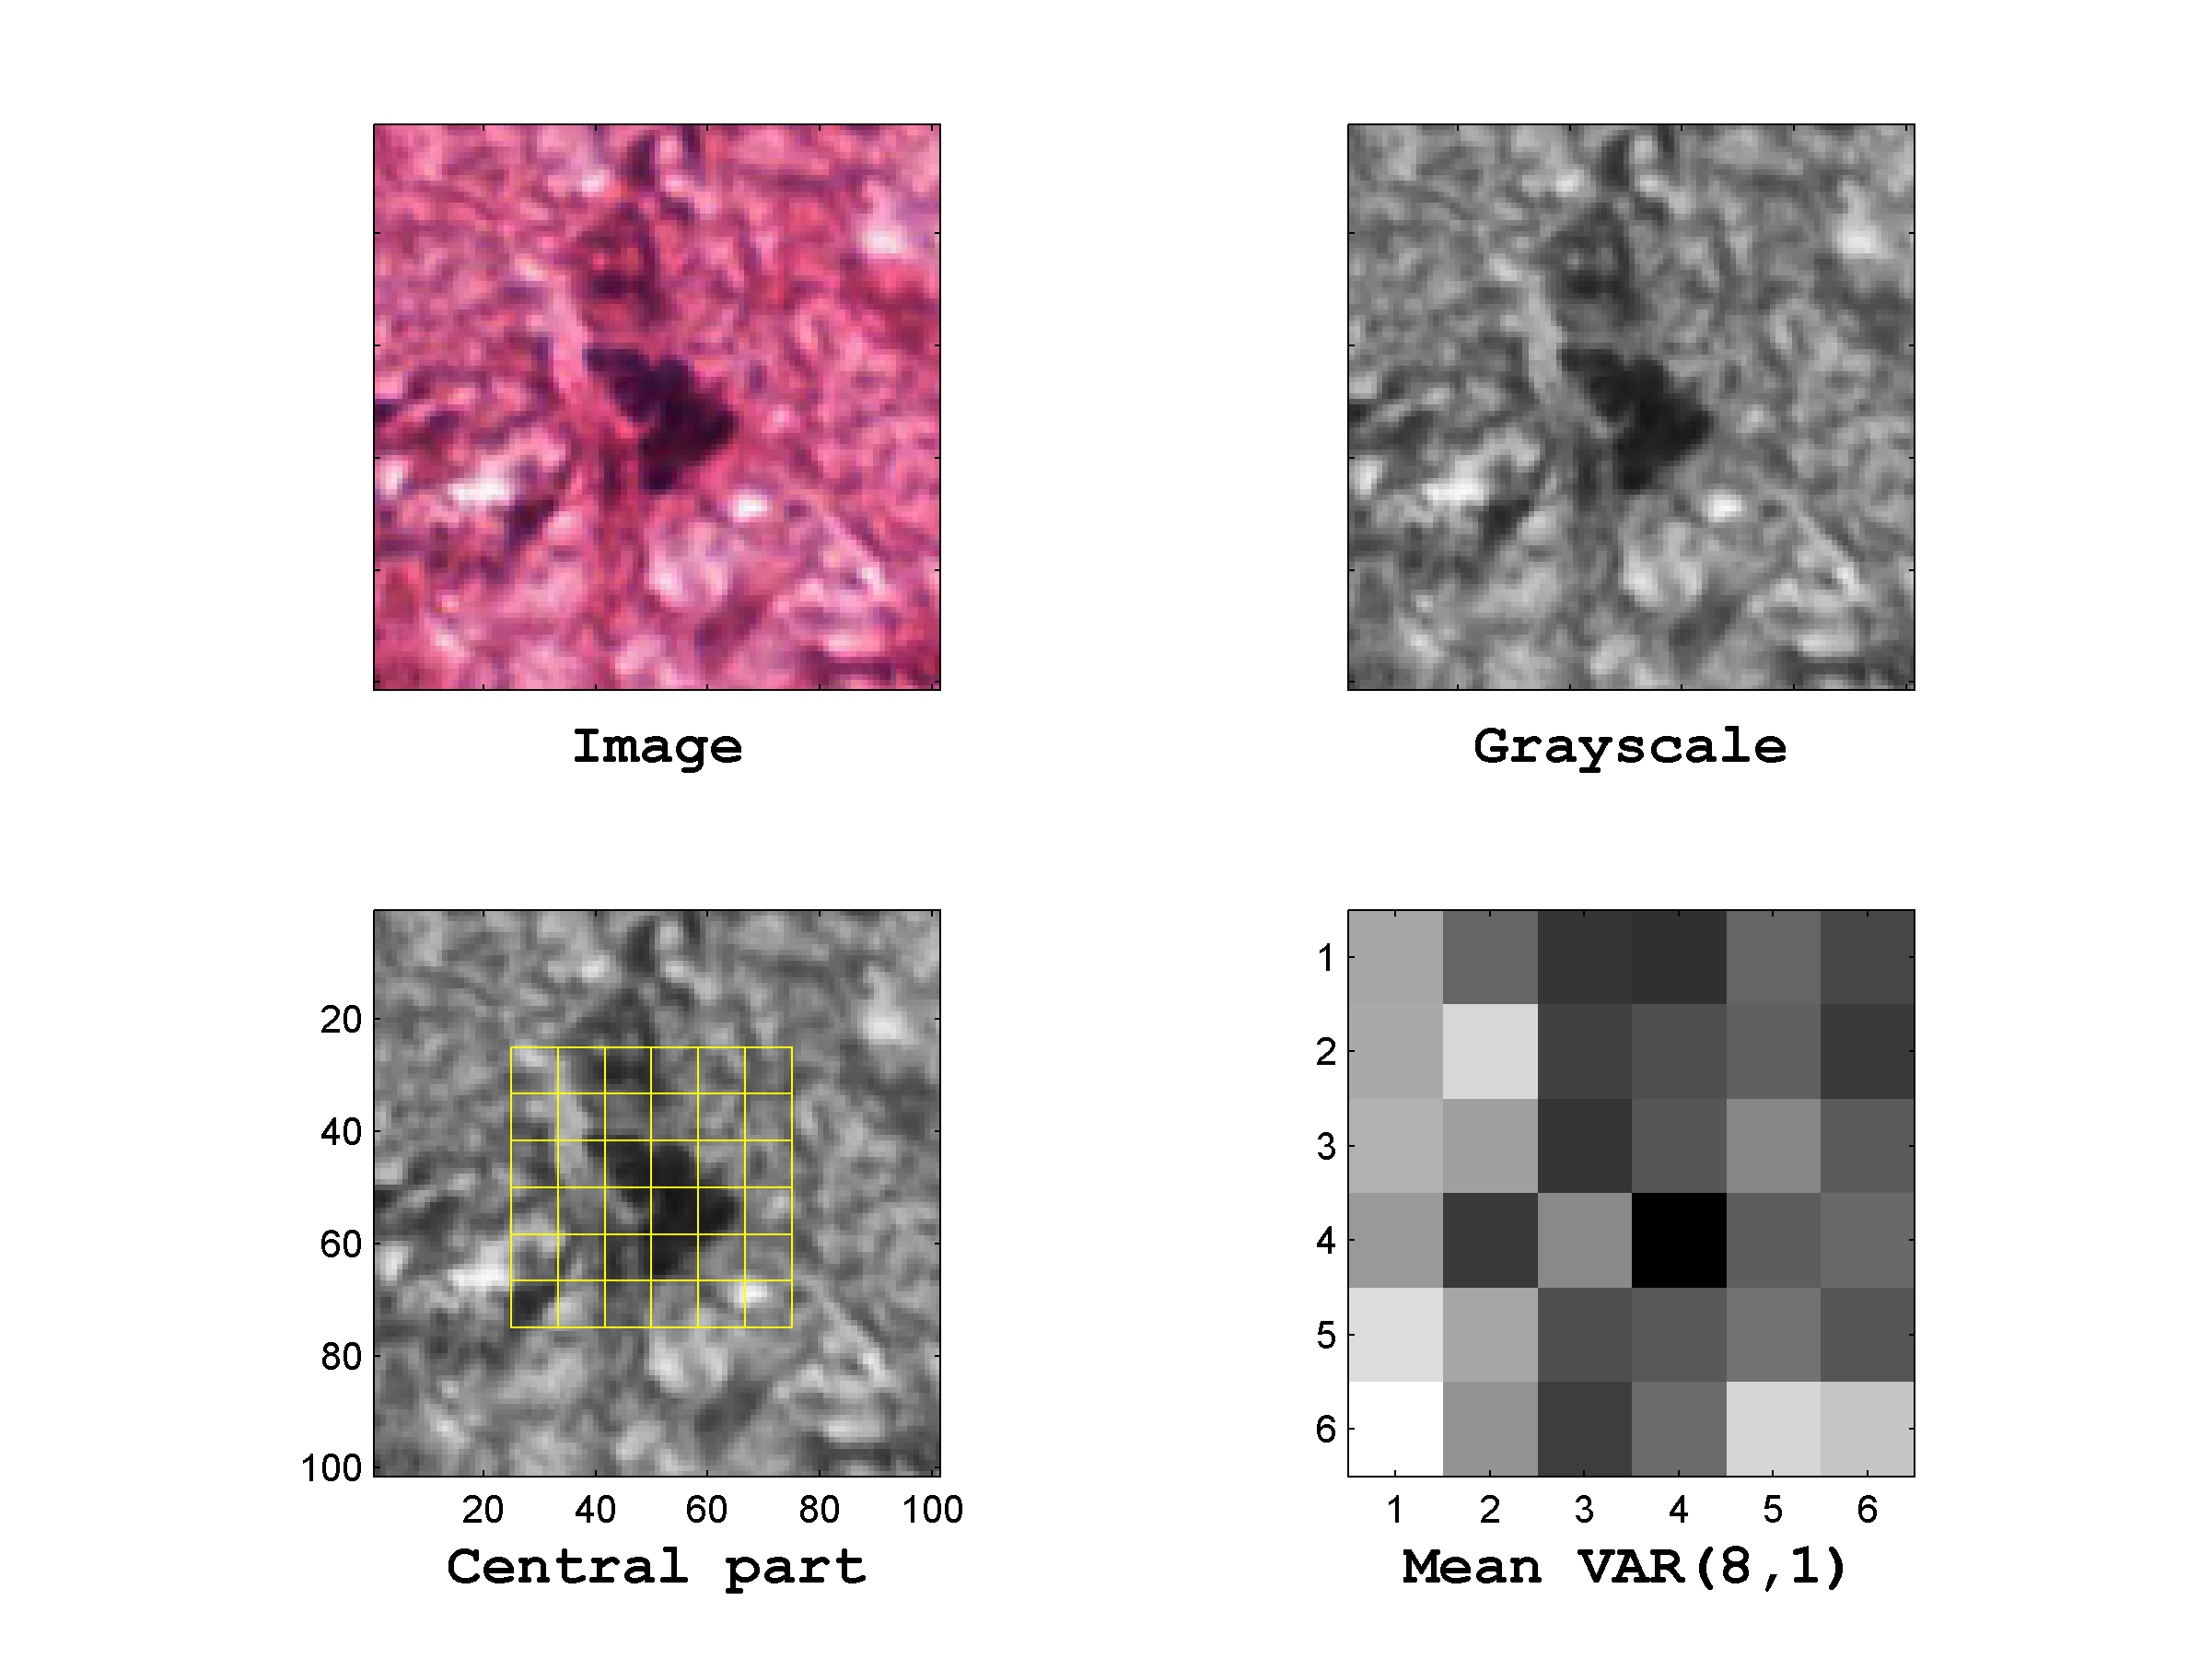
\includegraphics[width=0.94\textwidth]{./images/GS_VAR.png}
  \caption[Example of VAR(8,1) feature]{Example of VAR(8,1) feature}
  \label{ch4:fig4}
\end{figure}

The resulting feature vector is composed of 36 values, corresponding to the average VAR(8,1) in each element of the grid, ordered columnwise. This type of feature is orientation dependent.
\\
The Matlab code implemented to build the feature vectors is listed in \ref{appendixB:FE}


% \clearpage

%	-	l: lbp riu2 radius 1, 8 neighbors
%	-	r: lbp ri radius 1, 8 neighbors
%	-	u: lbp u2 radius 1, 8 neighbors
%	-	v: mean pixel variance
%	-	L: lbp riu2 radius 1-2-3, 8 neighbors concatenated
%	-	V: pixel variance, 36 elements
%	-	R: lbp ri radii 1-2-3, 8 neighbors
%	-	U: lbp u2 radii 1-2-3, 8 neighbors



\vspace{0.5cm}

%\clearpage

\section{Classifiers}
\label{ch4:classifiers}

Once defined the set of feature to be considered, it is possible to build a matrix whose lines represent an \textit{instance} (i.e. an image patch) and whose columns represent a \textit{feature}
(or a component of it): Equation \ref{ch4:fmat} represents such matrix.
\begin{equation}
\label{ch4:fmat}
 M_{feats} = \\ \bordermatrix{~ & \tikzmark{harrowleft} 1 & \cdots & ~  & \cdots & ~ & \cdots & ~ & n_{fc}\tikzmark{harrowright}  \cr
			      \tikzmark{varrowtop} 1 & c_{111} & c_{112} & \cdots & c_{1k1} & \cdots & c_{1kn_k} & \cdots & c_{1n_f1} \cr
			                      \vdots &    ~    &   ~     &   ~    &    ~    &   ~    &     ~     &    ~   &     ~     \cr
			                       ~     & \vdots  & \vdots  & \ddots & \vdots  & \ddots & \vdots    & \ddots &  \vdots   \cr
			                      \vdots &    ~    &   ~     &   ~    &   ~     &   ~    &    ~      &    ~   &    ~      \cr
			      \tikzmark{varrowbottom} n_i & \tikzmark{f1} c_{n_i11} & c_{n_i12} \tikzmark{f2} & \cdots & \tikzmark{f3} c_{n_ij1} & \cdots & c_{n_ijn_j} \tikzmark{f4} & \cdots & \tikzmark{f5} c_{n_in_f1} \tikzmark{f6} \cr
			     }
\end{equation}
\tikz[overlay,remember picture] {
  \draw[->] ([yshift=3ex]harrowleft) -- ([yshift=3ex]harrowright)
            node[midway,above] {\tiny \textit{features}};
  \draw[->] ([yshift=1.5ex,xshift=-0.8ex]varrowtop) -- ([xshift=-0.8ex]varrowbottom)
            node[pos=0.0,anchor=north,xshift=-0.65cm,yshift=-2.3cm] {\tiny \textit{instances}};
  \draw [thick, decoration={ brace, amplitude=8pt, mirror, raise=0.12cm}, decorate] (f1) -- (f2) 
	    node [pos=0.5,anchor=north,yshift=-0.36cm] {\tiny \textit{feat$_1$}};
  \draw [thick, decoration={ brace, amplitude=8pt, mirror, raise=0.12cm}, decorate] (f3) -- (f4) 
	    node [pos=0.5,anchor=north,yshift=-0.36cm] {\tiny \textit{feat$_j$}};
  \draw [thick, decoration={ brace, amplitude=5pt, mirror, raise=0.12cm}, decorate] (f5) -- (f6) 
	    node [pos=0.5,anchor=north,yshift=-0.36cm] {\tiny \textit{feat$_{nf}$}};
}

Where $n_f$ is the total number of features and $n_i$ is the total number of instances. Each feature can be made of more than one component (e.g. $feat_1$ and $feat_j$ in the example).
For this reason, the total number of columns in the matrix $(n_{fc})$ is given by the sum of all the feature components. So, 
each element of the matrix $c_{ijk}$ is the $k^{th}$ component of the $j^{th}$ feature in the $i^{th}$ instance. The matrix representing the eavluation set is built in the same way.\\
A vector represents the class which every instance belongs to. Equation \ref{ch4:cvect} describes such vector:
\begin{equation}
\label{ch4:cvect}
 V_{class} = \\ \bordermatrix{~ &  ~  \cr
			      \tikzmark{varrowtop} 1 &  \tikzmark{f5} e_{1}  \tikzmark{f6} \cr
			                      \vdots & \vdots \cr
			                       ~     & e_i   \cr
			                      \vdots & \vdots \cr
			      \tikzmark{varrowbottom} n_i & e_{n_i} \cr
			     }
\end{equation}
\tikz[overlay,remember picture] {
  \draw[->] ([yshift=1.5ex,xshift=-0.8ex]varrowtop) -- ([xshift=-0.8ex]varrowbottom)
            node[pos=0.0,anchor=north,xshift=-0.65cm,yshift=-2.3cm] {\tiny \textit{instances}};
  \draw [thick, decoration={ brace, amplitude=3pt, raise=0.25cm}, decorate] (f5) -- (f6) 
	    node [pos=0.5,anchor=north,yshift=0.76cm] {\tiny \textit{class}};
}

where $e_i$ belongs to one of the two classes. In some implementations of binary classifiers it is required that $e_i \ \in \{-1,1\} \ \forall i = 1,\cdots,n_i$,
otherwise $e_i \ \in \{0,1\} \ \forall i = 1,\cdots,n_i$. The vector 
representing the \Gls{GT} of the evaluation set is built in the same way.\\
Having a matrix representing the training feature set, a matrix representing the evaluation (i.e. testing) feature set and two vectors including the \Gls{GT}
classification of each image patch, it is possible to run a classifier that tries to get insights form the feature set in order to classify the evaluation set.\\


In our work we focused on two types of classifiers:

\begin{itemize}
 \item \textit{Support Vector Machines}, which are widely used in computer vision classification problems, in particular
in biomedical imaging (\cite{mitosisDetectionLearningBased, SVM02, SVM03, SVMClassHistogram}, see also Section \ref{ch3:review}),
 \item \textit{Random Forests}, which is a relatively new ensemble approach that can also be thought of as a form of nearest neighbor predictor (\cite{randForests03,randForests02,randForests04}).
\end{itemize}

We also mention \Gls{CNN}, as it played a relevant role in the definition of our dataset (see Section \ref{ch4:ic}).


\vspace{0.5cm}

\subsection{Support Vector Machines}
\label{ch4:svm}

We used the Matlab implementation of the \textit{libSVM} described in \cite{SVM01}. \Glspl{SVM} are a popular classification technique.
The goal of \Gls{SVM} is to produce a model (based on the training data) which predicts the target values of the test data
given only the test data attributes. Given a training set of instance-label pairs $(\mathbf{x_i}, y_i)$, $i = 1,\cdots,l$, where $\mathbf{x_i} \in \mathbb{R}^n$ and $y \in \{-1,1\}^l$.\\
The \Gls{SVM} requires the solution of the following optimization problem:

\begin{equation}
     \begin{aligned}
      \smash{\min_{\textbf{w},b,\xi}} \quad & \frac{1}{2}\textbf{w}^T\textbf{w}+C \sum_{i=1}^{l}\xi_i   \\
      \text{Subject to:} &\\
       & y_i \left(\textbf{w}^T \phi( \mathbf{x_i} ) +b\right) \geq 1-\xi_i \\
       & \xi_i \geq 0 
     \end{aligned}
     \phantom{\hspace{3cm}} %%<---adjust the value as you want
\end{equation}

The training vectors $\mathbf{x_i}$ are mapped into a higher dimensional space (maybe infinite), by the function $\phi$.
\Gls{SVM} finds a linear separating hyperplane with the maximal margin in this higher dimensional space.
$C > 0$ is the penalty parameter of the error term.
The function

\begin{equation}
 K(\mathbf{x_i}, \mathbf{x_j}) = \phi(\mathbf{x_i})^T\phi(\mathbf{x_j})
\end{equation}

is called the \textit{kernel function}. Many kernel functions have been defined, the most common are:

\begin{itemize}
 \item \textit{linear}: $K(\mathbf{x_i}, \mathbf{x_j}) = \mathbf{x_i}^T\mathbf{x_j}$,
 \item \textit{polynomial}: $K(\mathbf{x_i}, \mathbf{x_j}) = \left(\gamma \mathbf{x_i}^T\mathbf{x_j} + r \right)^d, \gamma > 0$,
 \item \textit{\Gls{RBF}}: $K(\mathbf{x_i}, \mathbf{x_j}) = \exp{\left(-\gamma \lVert \mathbf{x_i} - \mathbf{x_j} \rVert^2 \right)}, \gamma > 0$,
 \item \textit{sigmoid}: $K(\mathbf{x_i}, \mathbf{x_j}) = \tanh \left( \mathbf{x_i}^T\mathbf{x_j} + r \right)$.
\end{itemize}

Where $\gamma$, \textit{d} and \textit{r} are kernel parameters \cite{ML01}.\\
In our work we focused on \Glspl{RBF} and sigmoid kernels, which are used in most cases.
In \Glspl{SVM} the \textit{support vectors} are the training instances that concur to define the separating hyperplane in the kernel space. The 
image of Figure \ref{ch4:fig5} gives a linear representation of a \Gls{SVM}.

\begin{figure}[!hbt]
  \centering
    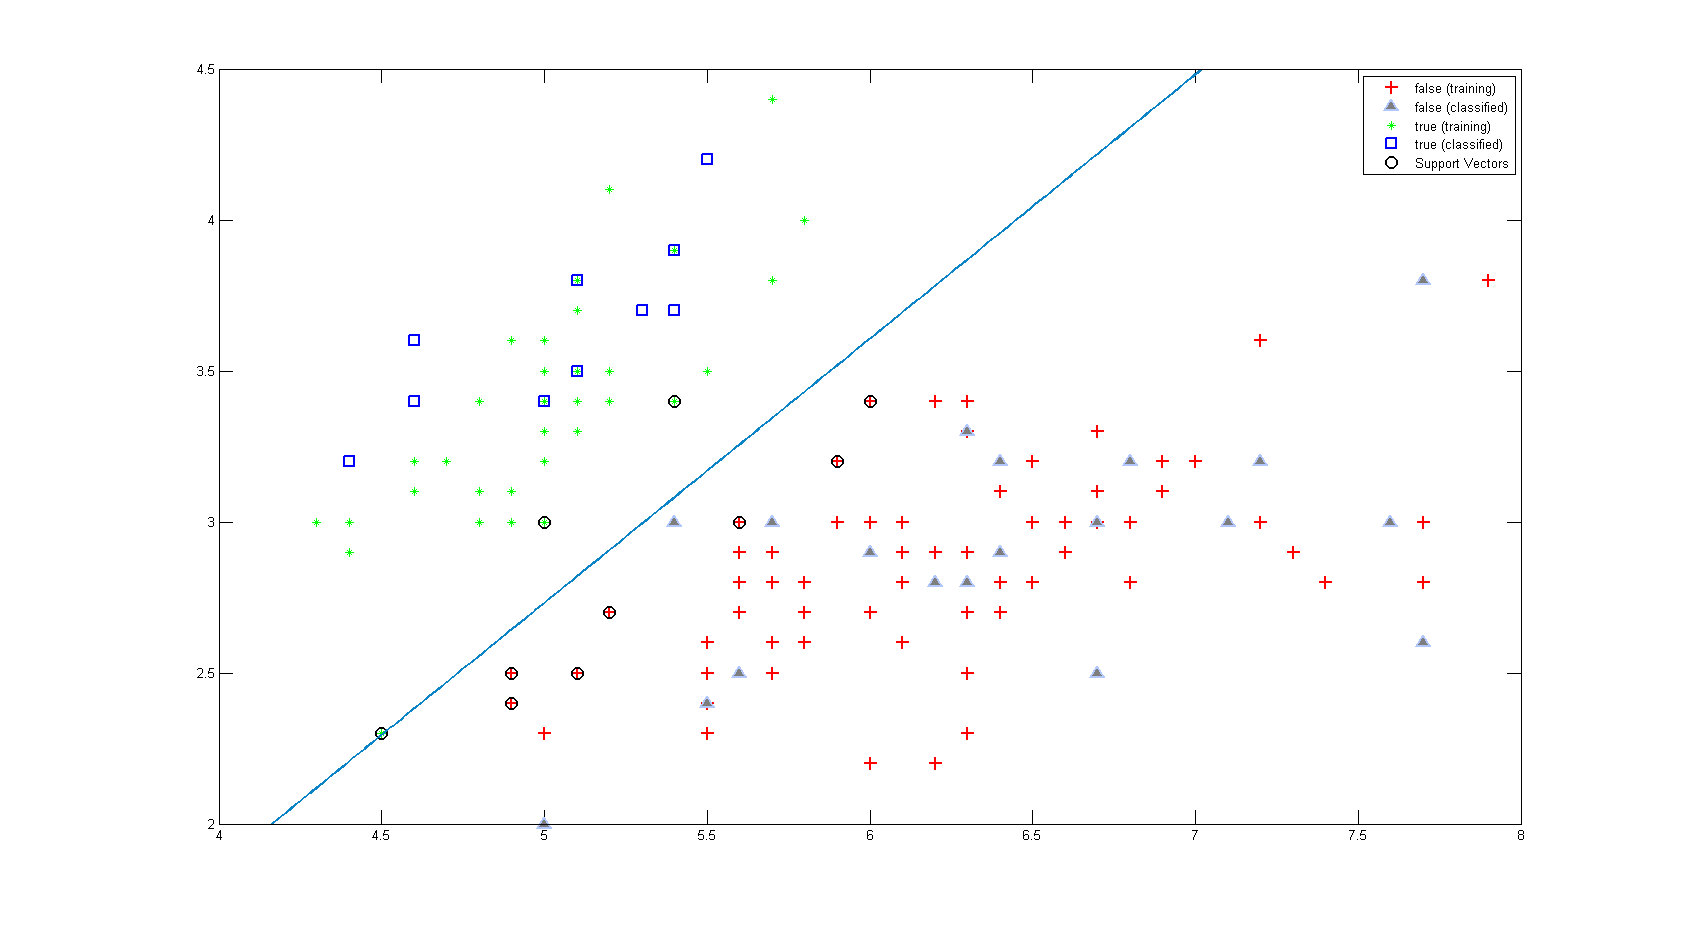
\includegraphics[width=0.98\textwidth]{./images/SVM_example.png}
  \caption{Representation of a SVM}
  \label{ch4:fig5}
\end{figure}


\vspace{0.5cm}

\subsection{Random Forests}

\Glspl{DT} are attractive classifiers due to their high execution speed and simplicity. However, trees often suffer from performance loss, in terms
of generalization accuracy on unseen data when the complexity of the problem grows \cite{randForests01}.\\
Random Forests are a combination of tree predictors such that each tree depends on the values of a
random vector sampled independently and with the same distribution for all trees in the forest \cite{randForests03}.
So, \Gls{RF} can be viewed as an ensemble approach that can also be thought of as a form of nearest neighbor predictor.
Ensembles are a divide-and-conquer approach used to improve performance. The main principle behind ensemble methods is that a group of \textquotedblleft weak learners\textquotedblright
can be combined together to form a \textquotedblleft strong learner\textquotedblright. Each classifier, individually, is a weak learner, while all the classifiers taken together are a strong learner.
An example of \Gls{DT} is shown in Figure \ref{ch4:fig6}.

\begin{figure}[!hbt]
  \centering
    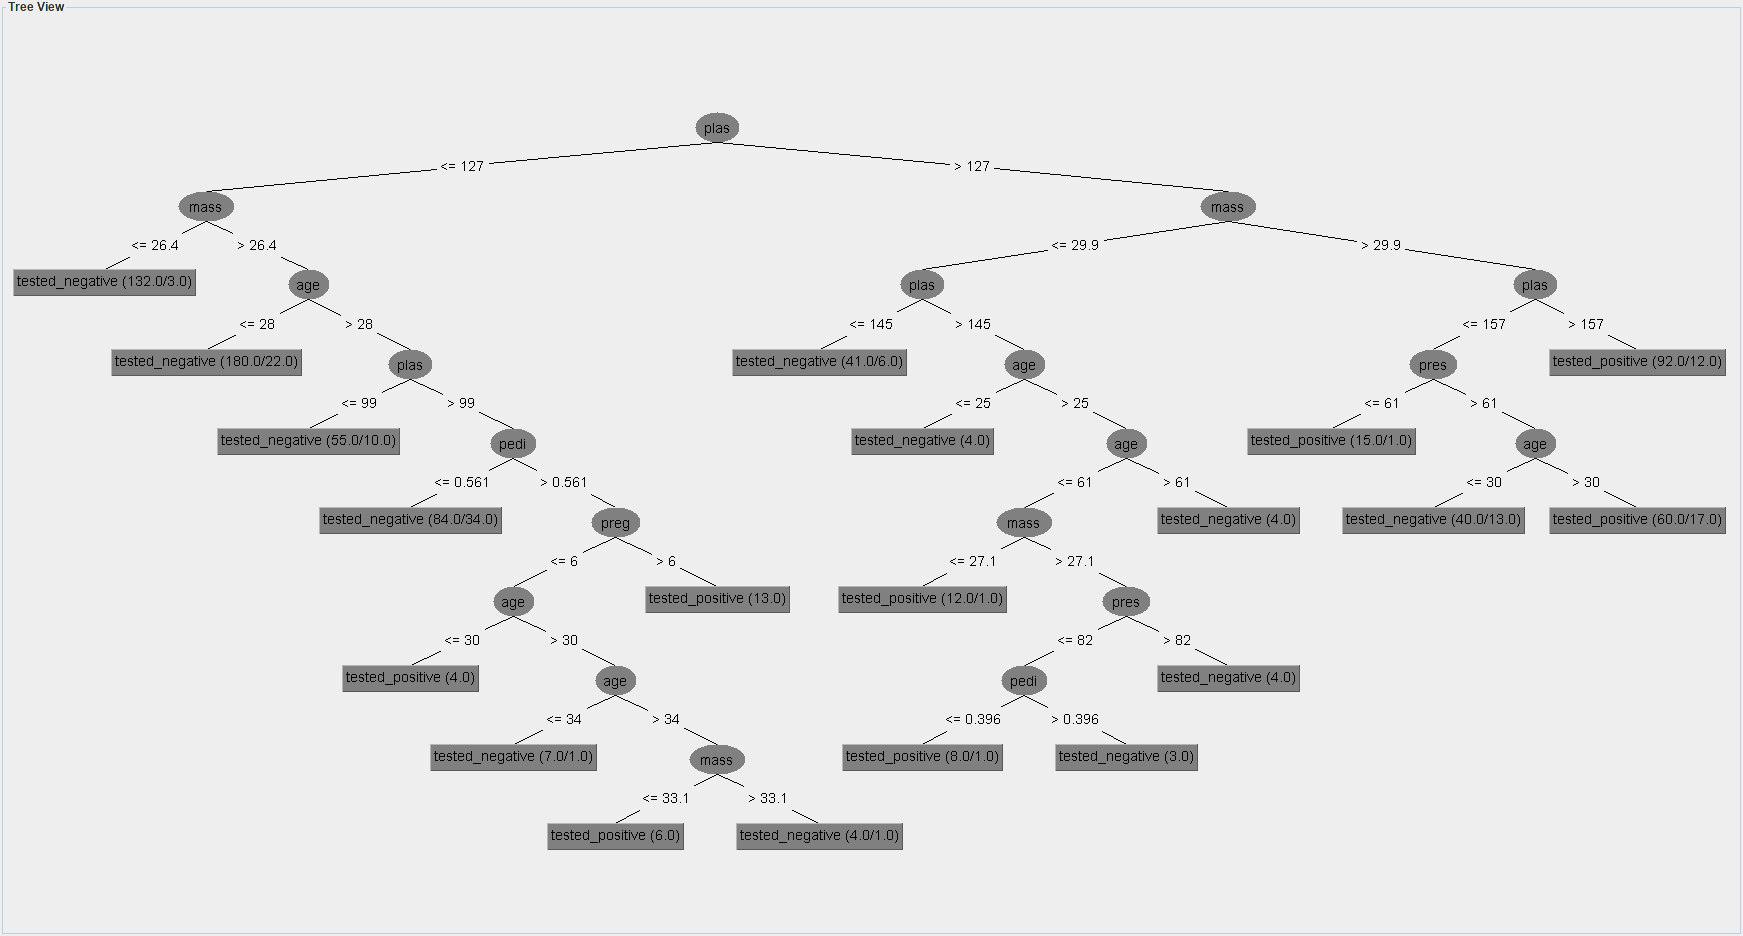
\includegraphics[width=0.98\textwidth]{./images/DT_example.png}
  \caption{Example of a Decision Tree}
  \label{ch4:fig6}
\end{figure}

A \Gls{RF} is composed by a number of trees \textbf{T}. For some number \textit{m}, \textit{m} features are randomly selected from the feature vector.
The subset of variables is used to train a \Gls{DT}.\\
According to Breiman implementation of \Glspl{RF}, \textit{m} should be that  $\ll$ than the number of features.\\
We adopted the convention in \cite{randForests03} that $m \leq \log_2 F +1$ and used an ensemble of 500 trees.\\
Running a \Gls{RF},when a new input is entered into the system (a test sample), it is run down all of the trees, each of which classifies
it in a \textquotedblleft hard\textquotedblright way (see \ref{ch3:class}): in a sense, each tree gives a vote for the current sample. 
The result is the average  of all of the terminal nodes that are reached, giving a final \textit{soft} classification.
\Glspl{RF} are generally quite fast, robust classifiers, and are also used in image classification \cite{randForests04}.
\\
The Matlab code implemented to classify data is listed in \ref{appendixB:Cl}.

\vspace{0.5cm}


\section{Classification Process}

Once a classifier is trained on the training set, it can be used to classify unseen data (i.e., the evaluation or testing set). The classifier
function is applied to each instance of the \textit{evaluation} feature set, which is built as the matrix described in Equation \ref{ch4:fmat}.\\
The output of the classifier is a vector like the one described in Equation \ref{ch4:cvect}, unless that, generally, the classification
process gives a \textit{soft} classification (see Section \ref{ch3:class}), which means that  $-1 \leq e_i \leq 1 \ \forall i = 1,\cdots,n_i$, or
$0 \leq e_i \leq 1$, depending on the definition of the classes.\\
The performance parameters are computed as a function of a \textit{classification threshold}, as described in Section \ref{ch3:roc}.



% In most computer vision applications it is not sufficient to extract only one type of feature to obtain the relevant information from the image data.
% Instead two or more different features are extracted, resulting in two or more feature descriptors at each image point.
% A common practice is to organize the information provided by all these descriptors as the elements of one single vector,
% commonly referred to as a feature vector. The set of all possible feature vectors constitutes a feature space.
% A common example of feature vectors appears when each image point is to be classified as belonging to a specific class.
% Assuming that each image point has a corresponding feature vector based on a suitable set of features,
% meaning that each class is well separated in the corresponding feature space, the classification of each image point can be done using standard classification method.

 


